% ============================================================
%  CHAPITRE 2 — Section 2 : Définition des indicateurs de performance
% ============================================================

\section{Définition des indicateurs de performance}
\label{sec:indicateurs}

Afin d'évaluer et de comparer les différentes EMS dans le cadre proposé, il est nécessaire de disposer d'indicateurs de performance bien définis, capables de rendre compte de la qualité du service rendu aux utilisateurs, de l'impact de la stratégie sur la durée de vie des composants, et de la résilience du système face aux aléas. Ces trois dimensions correspondent respectivement aux objectifs de court, long et moyen terme introduits dans la section précédente, et elles évoluent sur des échelles de temps fondamentalement différentes. Trois indicateurs complémentaires sont donc introduits~: la probabilité de coupure d'alimentation (LPSP), qui quantifie la fiabilité à court terme~; un coût de dégradation agrégé, qui chiffre l'usure à long terme induite par les décisions de contrôle~; et un indicateur de robustesse, qui mesure le service maintenu (au sens de la LPSP) lors d'une défaillance temporaire de composant. Les deux premiers indicateurs sont définis ci-dessous puis exploités dans le plan de Pareto tout au long du chapitre~; le troisième, dont la définition et le protocole d'évaluation sont établis ici, est mis en œuvre à la section~\ref{sec:robustesse}.

% ------------------------------------------------------------
\subsection{LPSP}
% ------------------------------------------------------------

Dans le contexte de cette étude, la qualité du service est évaluée strictement du point de vue de la continuité d'alimentation du consommateur. L'attention est donc portée sur le déficit de puissance. Les situations de surplus énergétique, dans lesquelles la production renouvelable excède à la fois la demande de charge et la capacité de charge des systèmes de stockage, communément appelées écrêtage (\textit{curtailment}), ne sont pas directement pénalisées par cet indicateur. Il est supposé que, durant ces intervalles, la stratégie de contrôle adapte l'algorithme de suivi du point de puissance maximale (MPPT) afin d'écrêter la production solaire, maintenant ainsi la stabilité du bus continu sans affecter la fourniture d'énergie à la charge.

L'indicateur retenu pour quantifier la fiabilité est la \textit{Loss of Power Supply Probability} (LPSP). Cette métrique est largement adoptée dans la littérature traitant de la gestion d'énergie et du dimensionnement des systèmes d'énergie renouvelable hybrides~\cite{korovushkin_modern_2025}\cite{heydari_combined_2023}. La LPSP est définie comme la fraction de la demande totale en énergie qui ne peut pas être satisfaite par le système hybride sur un horizon de temps donné. Elle varie entre 0 et 1~: une valeur de 0 signifie que la charge est intégralement satisfaite à tout instant, tandis qu'une valeur de 1 correspond à une charge jamais satisfaite. Mathématiquement, la LPSP s'exprime comme le rapport entre le déficit énergétique cumulé et la demande énergétique totale sur l'ensemble de la période de simulation~:

\begin{equation}
    \mathrm{LPSP} = \frac{\sum_{t} \mathrm{LPS}(t)\cdot \Delta t}{\sum_{t} \hat{P}_{\text{Load}}(t) \cdot \Delta t}
    \label{eq:lpsp}
\end{equation}

où $\mathrm{LPS}(t)$ [W] représente la perte de puissance d'alimentation à l'instant $t$, définie comme~:

\begin{equation}
    \mathrm{LPS}(t) =
    \begin{cases}
      \hat{P}_{\text{Load}}(t) - P_{\text{Avail}}(t) & \text{si } \hat{P}_{\text{Load}}(t) > P_{\text{Avail}}(t) \\
      0 & \text{sinon}
    \end{cases}
    \label{eq:lps}
\end{equation}

où $\hat{P}_{\text{Load}}(t)$ [W] est la puissance demandée par la charge à l'instant $t$, et $P_{\text{Avail}}(t)$ [W] est la puissance totale disponible auprès de la production PV et des systèmes de stockage à cet instant.

% ------------------------------------------------------------
\subsection{Robustesse face aux défaillances}
\label{subsec:indic_robustesse}
% ------------------------------------------------------------

La LPSP rend compte de la qualité du service en régime nominal, lorsque tous les composants sont opérationnels. Un micro-réseau isolé est toutefois, par construction, dépourvu de secours extérieur~: la défaillance temporaire d'un organe de stockage (défaut d'un module hydrogène, déclenchement d'une protection, opération de maintenance...) peut survenir en cours d'exploitation et compromettre la continuité de service. Cette dimension relève d'une échelle de temps intermédiaire, entre la dynamique horaire du suivi de charge et la dynamique pluriannuelle du vieillissement~: une panne dure typiquement de quelques heures à quelques jours, le temps de la réparation. Un tel régime dégradé n'est rendu par aucun des indicateurs de fonctionnement nominal, ni la fiabilité ni la durabilité, et appelle donc une métrique propre.

Les défaillances considérées ici ne portent que sur les composants hydrogène (PEMFC et PEMWE). Les données de fiabilité de terrain (\textit{Mean Time Between Failure (MTBF), Mean Time To Failure (MTTF)...}) restent rares et difficiles à unifier, les trois technologies ne se prêtant à aucun référentiel commun, mais leur triangulation à partir de sources disponibles (relevés de terrain pour la batterie~\cite{ieee_std_493_2007}, feuilles de route technico-économiques pour la pile à combustible~\cite{fch2ju_mawp_2018}, analyse par arbre de défaillances pour l'électrolyseur~\cite{ubale_failure_2025}) fait apparaître un écart de deux à trois ordres de grandeur~: les défaillances de la batterie sont beaucoup plus rares que celles des composants hydrogène. Il est donc cohérent de concentrer l'analyse sur ces derniers, la batterie jouant alors le rôle de réserve de repli.

Une défaillance est modélisée comme l'indisponibilité temporaire d'un composant hydrogène, survenant à un instant $t_0$ et réparée au bout d'une semaine ($\Delta t_{\text{panne}} = \SI{168}{\hour}$). Deux sévérités sont retenues~: la défaillance totale (puissance du composant ramenée à \SI{0}{\percent}) et la défaillance partielle (puissance maximale dégradée à \SI{50}{\percent}). Les piles à combustible et les électrolyseurs PEM sont des assemblages modulaires, si bien qu'un défaut localisé (cellule défaillante, \textit{stack} isolé par sa protection, auxiliaire de \textit{balance-of-plant} défaillant...) met hors service une fraction du composant sans l'arrêter complètement. Une perte de l'ordre de la moitié de la capacité constitue ainsi un mode de défaillance représentatif, et éprouve la capacité de l'EMS à exploiter la puissance résiduelle. Croisées avec les deux composants, ces sévérités définissent quatre scénarios~: PEMFC totale, PEMFC \SI{50}{\percent}, PEMWE totale et PEMWE \SI{50}{\percent}.

L'indicateur de robustesse est la LPSP subie en présence de la panne, mesurée sur une fenêtre d'évaluation $[t_0,\, t_0 + \Delta t_{\text{éval}}]$. Les dégradations des composants ne sont pas prioritaires dans ce cas puisqu'il est considéré que l'acheminement de puissance pour assurer le service aux usagers sur cette courte période est l'aspect central. Pour un scénario $\sigma = (c, \kappa)$, défini par le composant défaillant $c \in \{\text{PEMFC}, \text{PEMWE}\}$ et un facteur de sévérité $\kappa \in \{0\,;\,0{,}5\}$, la puissance maximale du composant $c$ est plafonnée à $\kappa\, P_{\text{max}}^{c}$ pendant la panne, puis rétablie à $P_{\text{max}}^{c}$ après réparation. Il en résulte une puissance disponible $P_{\text{Avail}}^{\sigma}(t)$, et donc une perte d'alimentation $\mathrm{LPS}^{\sigma}(t)$ au sens de l'équation~\eqref{eq:lps}. La LPSP sous défaillance s'écrit alors~:
\begin{equation}
    \mathrm{LPSP}_{\text{panne}}^{\sigma}(t_0) = \frac{\displaystyle\sum_{t=t_0}^{t_0+\Delta t_{\text{éval}}} \mathrm{LPS}^{\sigma}(t)\cdot \Delta t}{\displaystyle\sum_{t=t_0}^{t_0+\Delta t_{\text{éval}}} \hat{P}_{\text{Load}}(t)\cdot \Delta t}
    \label{eq:lpsp_panne}
\end{equation}
La fenêtre d'évaluation est volontairement plus longue que la panne~: $\Delta t_{\text{éval}} = 4\,\text{semaines}$, soit la semaine de défaillance suivie de trois semaines de reprise post-réparation. Cet allongement est nécessaire pour capturer le coût différé des pannes d'électrolyseur~: pendant l'indisponibilité du PEMWE, le surplus PV non électrolysé recharge la batterie et masque temporairement le déficit~; le vrai coût, un réservoir d'hydrogène appauvri et donc une pile à combustible en sous-alimentation, n'apparaît qu'après la réparation.

L'instant de panne $t_0$ étant a priori inconnu, il est traité comme une variable aléatoire de loi uniforme sur la période d'exploitation. L'indicateur de robustesse d'une stratégie $s$ pour le scénario $\sigma$ est alors défini comme l'espérance de la LPSP subie sous défaillance, estimée par la moyenne empirique sur $N$ instants de panne $t_0^{(n)}$~:
\begin{equation}
    R^{\sigma}(s) = \mathbb{E}_{t_0}\!\big[\mathrm{LPSP}_{\text{panne}}^{\sigma}(t_0)\big] \;\approx\; \frac{1}{N}\sum_{n=1}^{N} \mathrm{LPSP}_{\text{panne}}^{\sigma}\!\big(t_0^{(n)}\big),
    \label{eq:indic_robustesse}
\end{equation}
une stratégie étant d'autant plus robuste que $R^{\sigma}(s)$ est faible. À titre de diagnostic complémentaire, le surcoût de robustesse peut être rapporté~; il mesure l'écart à la LPSP qu'aurait connue la même stratégie sur la même fenêtre en l'absence de panne~:
\begin{equation}
    \Delta \mathrm{LPSP}_{\text{rob}}(t_0) = \mathrm{LPSP}_{\text{panne}}^{\sigma}(t_0) - \mathrm{LPSP}_{\text{nominal}}(t_0),
    \label{eq:surcout_robustesse}
\end{equation}
qui isole l'effet propre de la défaillance de la variabilité du profil de charge.

L'estimation de cette espérance repose sur une expérience de Monte-Carlo conçue pour isoler le comportement propre de chaque stratégie face à une panne, toutes choses égales par ailleurs. Une trajectoire de fond commune est d'abord établie en simulant sur deux ans la stratégie de référence RB2 (section~\ref{sec:resultats}), afin d'atteindre un régime permanent réaliste. Cette trajectoire fournit, à chaque heure, un instantané complet de l'état du système~: SoC de la batterie, niveau du réservoir d'hydrogène $E_{\text{H2}}$, états de santé et de vieillissement des composants. Le premier mois (environ 730~h) sert à établir ce régime permanent et est exclu des instants de panne, si bien que les instants $t_0^{(n)}$ sont tirés dans les mois 2 à 24. Partir d'une même trajectoire de fond garantit que toutes les stratégies sont éprouvées depuis un même état initial, ce qui rend la comparaison équitable.

À l'instant $t_0$, la simulation repart de cet instantané et déroule la fenêtre d'évaluation, le vieillissement étant gelé car négligeable à l'échelle de quelques semaines. La panne est supposée détectée par l'EMS~: à chaque pas, la stratégie évaluée calcule son intention de répartition normale, puis la puissance du composant défaillant est plafonnée à sa capacité disponible $\kappa\,P_{\text{max}}^{c}$ et le manque est rerouté vers la batterie. Les contraintes physiques du modèle, qui gèrent la saturation du SoC et du réservoir d'hydrogène, fixent enfin la puissance effectivement servie.

Le nombre de tirages est fixé à $N = 200$, les instants étant identiques pour toutes les stratégies et tous les scénarios, de sorte que la comparaison soit appariée et non polluée par le bruit d'échantillonnage. Ce protocole est résumé à la Figure~\ref{fig:rob_methodo}. Les stratégies ainsi évaluées sont les neuf EMS comparées dans ce chapitre (section~\ref{sec:ems})~; leurs résultats de robustesse sont analysés à la section~\ref{sec:robustesse}.

\begin{figure}[h!]
    \centering
    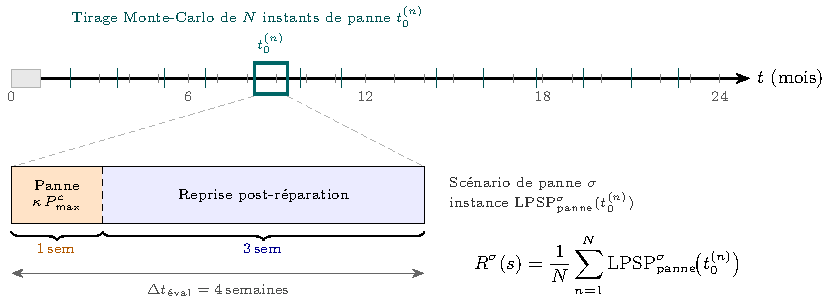
\includegraphics[width=\linewidth]{Chapitre 2/Robustesse/Figures/protocole_robustesse.pdf}
    \caption{Protocole d'évaluation de la robustesse par tirage Monte-Carlo des instants de panne.}
    \label{fig:rob_methodo}
\end{figure}
\FloatBarrier

% ------------------------------------------------------------
\subsection{Dégradations}
% ------------------------------------------------------------

Si la LPSP rend compte de l'adéquation à court terme du système, la performance à long terme est associée au taux de dégradation des principaux composants de stockage et de conversion. Ceux-ci sont soumis à des mécanismes d'usure directement liés aux décisions de l'EMS~: les cycles de charge et décharge de la batterie, les cycles de démarrage-arrêt des équipements hydrogène, les transients de puissance, ou encore les périodes de fonctionnement à forte charge. L'enjeu est donc de construire des indicateurs capables de quantifier cet impact de manière cohérente et comparable entre technologies.

L'indicateur de dégradation total $D_{\text{tot}}$ est défini comme la somme de trois sous-indicateurs normalisés correspondant respectivement à la batterie, à la pile à combustible (PEMFC) et à l'électrolyseur (PEMWE)~:

\begin{equation}
    D_{\text{tot}} = C_{\text{bat}} D_{\text{bat}}^{*} + C_{\text{FC}} D_{\text{FC}}^{*} + C_{\text{ELY}} D_{\text{ELY}}^{*}
    \label{eq:degradation_total}
\end{equation}

où les termes $D^{*}$ représentent des indices de dégradation normalisés (sans dimension), et les coefficients $C$ correspondent à des pondérations proportionnelles aux coûts de remplacement des composants. La normalisation est effectuée par rapport au critère de fin de vie (EoL, \textit{End of Life}) de chaque composant, de sorte que chaque $D^{*}$ prenne ses valeurs entre 0 (composant neuf) et 1 (composant en fin de vie). Les critères de fin de vie retenus sont respectivement une perte de capacité de \SI{30}{\percent} pour la batterie (soit un SoH de \SI{70}{\percent}), et une augmentation ou une perte de \SI{10}{\percent} de la puissance à courant constant pour l'électrolyseur et la pile à combustible. Le seuil batterie est cohérent avec la pratique courante en stationnaire, où la fin de vie est généralement placée entre 70 et \SI{80}{\percent} de la capacité initiale~\cite{madani_comprehensive_2025}~; la valeur retenue ici se situe sur le bord conservateur de cet intervalle, et il sera montré à la section~\ref{sec:sensibilite} que le classement qualitatif des stratégies y est insensible. La structure de cet indicateur agrégé, le calcul de chaque contribution physique et le choix des pondérations sont détaillés dans les sous-sections suivantes.

% - - - - - - - - - - - - - - - - - - - - - - - - - - - - - -
\subsubsection{Batteries}
% - - - - - - - - - - - - - - - - - - - - - - - - - - - - - -

L'indicateur de dégradation de la batterie $D_{\text{bat}}$ développé dans cette sous-section estime un niveau de vieillissement en fonction du profil de puissance appliqué à la batterie.  

Conformément à la littérature et aux développements de Maheshwari \textit{et al.}~\cite{maheshwari_optimizing_2020}, la dégradation par cyclage dépend de trois facteurs de stress physiques majeurs et interconnectés~: le niveau de l'état de charge (SoC, \textit{State of Charge}), la profondeur de décharge (DoD, \textit{Depth of Discharge}) des cycles effectués, et le régime de courant appliqué (C-rate)~\cite{madani_comprehensive_2025}\cite{asiri_impact_2025}. Le vieillissement calendaire est ici considéré comme indépendant des décisions de commande directes et n'est pas considéré ici où l'objectif est de quantifier l'impact d'un profil de puissance appliqué à une batterie. 

La première étape de la quantification consiste à projeter le profil de puissance externe sur les variables d'état internes de la batterie. Soit un profil temporel discret où chaque pas de temps $t$ est caractérisé par une puissance de charge $P_t^{ch}$ et une puissance de décharge $P_t^{dis}$. L'évolution de l'état de charge $\text{SoC}_t$ (exprimé en pourcentage) est régie par l'équation de bilan de matière suivante~\cite{maheshwari_optimizing_2020}~:
\begin{equation}
    \text{SoC}_t = \text{SoC}_{t-1} + \frac{(\eta \cdot P_t^{ch} - \frac{1}{\eta} \cdot P_t^{dis}) \cdot \Delta T}{V_{\text{nom}} \cdot I_{1\text{C}}} \times 100
    \label{eq:soc_evolution}
\end{equation}
où $\Delta T$ représente la durée du pas de temps, $V_{\text{nom}}$ désigne la tension nominale de la batterie (considérée comme constante pour découpler les variations de tension des effets directs du profil de puissance), et $I_{1\text{C}}$ correspond à l'intensité du courant nominal au régime de référence de 1C (en Ampères)~\cite{maheshwari_optimizing_2020}. Le paramètre $\eta$ représente le rendement d'efficacité de l'accumulateur, permettant de modéliser les pertes énergétiques internes lors des transferts de charge.

Pour s'affranchir des algorithmes classiques de comptage de cycles (tels que la méthode Rainflow), qui nécessitent une connaissance \textit{a posteriori} complète du profil et s'avèrent complexes à formaliser analytiquement, Maheshwari \textit{et al.}~\cite{maheshwari_optimizing_2020} introduisent le concept de fonction de dégradation cumulée dépendante du chemin. La dégradation de référence induite à un régime de courant standard de 1C est décrite par la courbe non linéaire $\delta^{1\text{C}}(\text{SoC})$ présentée à la Figure~\ref{fig:battery_deg}. Cette courbe associe un potentiel de dégradation virtuel (exprimé en $\mu\text{Ah}$) à chaque niveau de charge de la batterie. 

La dégradation élémentaire survenant au cours d'un pas de temps $t$, notée $d_t^{1\text{C}}$, est alors définie comme la variation absolue de ce potentiel entre le début et la fin de l'intervalle~\cite{maheshwari_optimizing_2020}~:
\begin{equation}
    d_t^{1\text{C}} = |\delta^{1\text{C}}(\text{SoC}_t) - \delta^{1\text{C}}(\text{SoC}_{t-1})|
    \label{eq:deg_step_1c}
\end{equation}
Cette formulation permet de capturer simultanément et de manière intrinsèque l'effet du SoC moyen d'utilisation et de la profondeur de décharge (DoD). Un cycle de grande amplitude (fort DoD) ou une sollicitation dans des zones de SoC à forte décharge (zones de contraintes chimiques intenses aux extrêmes de la courbe de la Figure~\ref{fig:battery_deg}) engendrera mécaniquement une variation plus élevée de la fonction, et donc une dégradation $d_t^{1\text{C}}$ plus importante~\cite{maheshwari_optimizing_2020}.

\begin{figure}[h!]
    \centering
    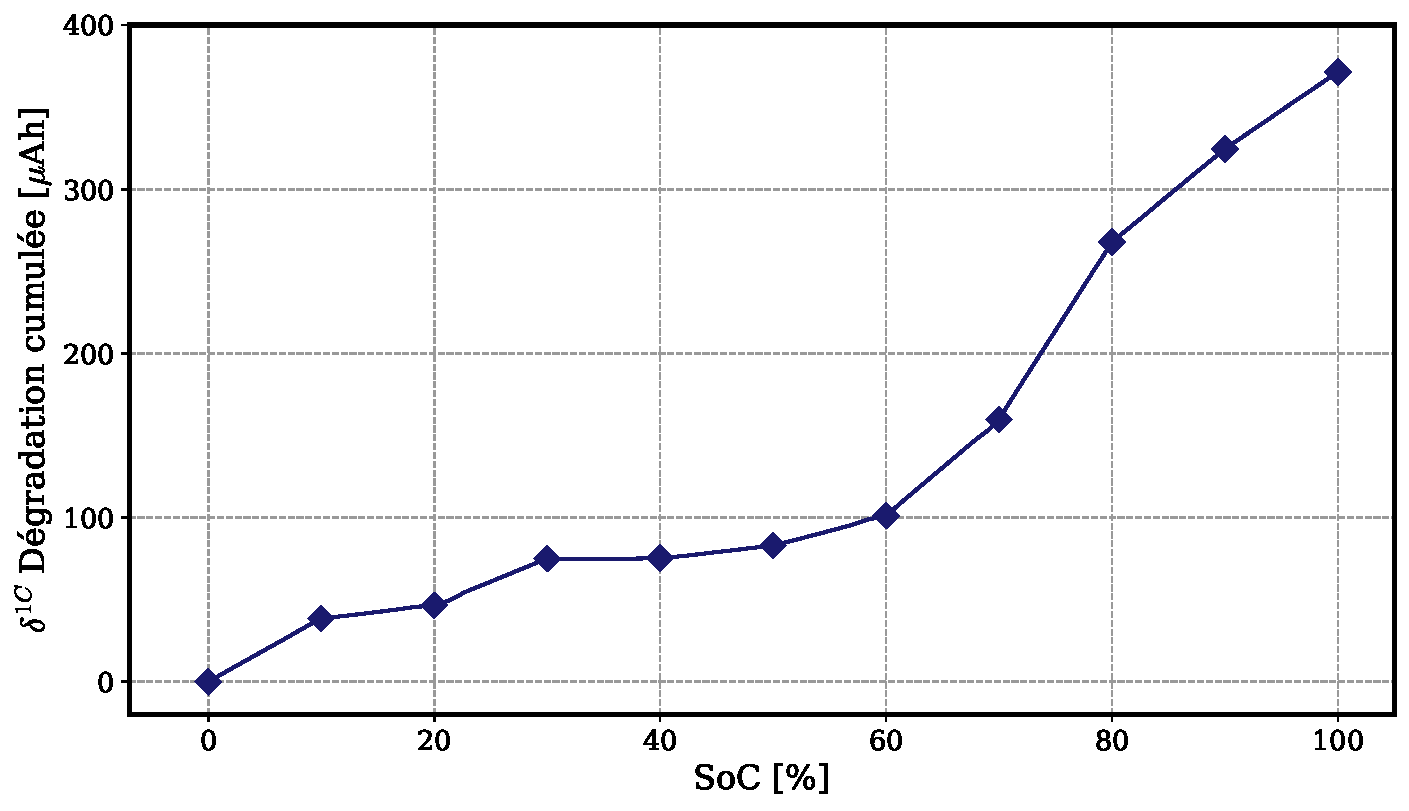
\includegraphics[width=0.8\linewidth]{Chapitre 2/Indicateurs/Figures/batt_deg_dod_cumul.pdf}
    \caption{Dégradation cumulée de la capacité de la batterie induite par le cyclage~\cite{maheshwari_optimizing_2020}.}
    \label{fig:battery_deg}
\end{figure}
\FloatBarrier

La dégradation de référence $d_t^{1\text{C}}$ doit ensuite être corrigée pour intégrer l'effet de l'intensité du courant réel (C-rate), qui accélère le vieillissement en accentuant les contraintes mécaniques (gradients de concentration de lithium, fissuration de l'interface d'électrolyte solide SEI) et les échauffements locaux. Le C-rate effectif $i_t$ auquel est soumis l'accumulateur au pas de temps $t$ est directement calculé à partir du profil de puissance~\cite{maheshwari_optimizing_2020}~:
\begin{equation}
    i_t = \frac{P_t^{ch} + P_t^{dis}}{V_{\text{nom}} \cdot I_{1\text{C}}}
    \label{eq:crate_calculation}
\end{equation}
L'impact de ce courant est modélisé de façon multiplicative par un facteur d'échelle empirique $\psi(i_t)$, indépendant de l'état de charge~\cite{maheshwari_optimizing_2020}. Ce facteur est normalisé pour valoir contractuellement 0 à circuit ouvert (0C, absence de courant de cyclage) et 1 au régime nominal de 1C. À partir des données expérimentales de l'étude d'origine, la progression de ce facteur est interpolée linéairement entre les points de contrôle empiriques pour refléter l'accroissement des dommages à fort régime~\cite{maheshwari_optimizing_2020}~:
\begin{equation}
    \psi(i_t) = 
    \begin{cases} 
      i_t & \text{si } 0 \le i_t \le 1 \\
      1 + 0{,}2956 \cdot (i_t - 1) & \text{si } 1 < i_t \le 2 
    \end{cases}
    \label{eq:psi_crate}
\end{equation}

En combinant l'influence géométrique du cycle (SoC et DoD) et l'intensité du courant, la dégradation effective subie par la batterie à chaque pas de temps, notée $\delta_t$, s'exprime sous la forme du produit fonctionnel suivant~\cite{maheshwari_optimizing_2020}~:
\begin{equation}
    \delta_t = d_t^{1\text{C}} \times \psi(i_t)
    \label{eq:effective_degradation_step}
\end{equation}

Finalement, l'indicateur de dégradation totale accumulée sur l'ensemble du profil de simulation, noté $D_{\text{bat}}$, est obtenu par la sommation directe de ces contributions temporelles~:
\begin{equation}
    D_{\text{bat}} = \sum_t \delta_t
    \label{eq:total_degradation}
\end{equation}

Exprimé de manière absolue en Ampères-heures (Ah) ou en pourcentage de capacité initiale amortie, cet indicateur $D_{\text{bat}}$ synthétise l'impact physique global du profil de puissance appliqué. Il constitue la grandeur d'entrée requise pour la suite des calculs de cette section~: en multipliant cette valeur de capacité perdue par le coût unitaire de remplacement de la batterie (exprimé en €/Ah perdu), il devient possible d'attribuer un coût financier précis, direct et objectif à n'importe quelle séquence opérationnelle imposée au système de stockage.

% - - - - - - - - - - - - - - - - - - - - - - - - - - - - - -
\subsubsection{Piles à combustible}
% - - - - - - - - - - - - - - - - - - - - - - - - - - - - - -

De même que pour les batteries, l'évaluation du coût d'exploitation d'une PEMFC requiert un formalisme capable de traduire un profil opérationnel de puissance en une mesure physique quantifiable du vieillissement. L'indicateur de dégradation globale de la pile à combustible, noté $D_{\text{FC}}$ et développé dans cette sous-section, remplit ce rôle en estimant le taux d'usure cumulé du système, exprimé sous la forme d'un pourcentage de perte de performance ou de chute de tension nominale.

Conformément aux travaux empiriques de Pei \textit{et al.}~\cite{pei_quick_2008} ainsi qu'aux analyses de Foniok \textit{et al.}~\cite{foniok_mechanisms_2025} et de Nguyen \textit{et al.}~\cite{nguyen_comprehensive_2023}, le vieillissement d'une PEMFC en conditions de transport ou de sollicitations stationnaires dynamiques ne dépend pas seulement du temps de fonctionnement linéaire, mais résulte de la superposition de quatre régimes opérationnels principaux et particulièrement contraignants~: les événements de démarrage-arrêt, les périodes de ralenti, les transitoires dynamiques de charge, et le fonctionnement prolongé à forte puissance. L'objectif est ici d'isoler ces contributions afin de quantifier l'état d'usure du système.

L'indicateur de dégradation totale $D_{\text{FC}}$ est ainsi modélisé par une formulation additive découplant l'impact de chacun de ces quatre mécanismes majeurs~\cite{pei_quick_2008}~:
\begin{equation}
    D_{\text{FC}} = d_{\text{start-stop}} + d_{\text{idling}} + d_{\text{transient}} + d_{\text{high power}}
    \label{eq:degradation_fc}
\end{equation}
La superposition additive de mécanismes, chacun affecté d'un taux de chute de tension indépendant, constitue un choix de modélisation répandu pour le vieillissement des PEMFC~\cite{nguyen_comprehensive_2023}\cite{foniok_mechanisms_2025}. Les taux élémentaires de chacune des quatre contributions sont ici calibrés à partir des données expérimentales de Song \textit{et al.}~\cite{song_pontryagins_2020} et exprimés en pourcentage de chute de tension.

Pour formaliser mathématiquement ces contributions sans recourir à des variables binaires d'optimisation, les équations sont définies de manière purement descriptive à partir de la série temporelle de la puissance électrique délivrée par la pile, notée $P_t$, sur un horizon temporel discret discrétisé par pas de temps $\Delta T$. 

La première contribution, $d_{\text{start-stop}}$, comptabilise l'impact des cycles de mise en marche et d'arrêt. Lors de ces phases transitoires, la formation temporaire d'un front hydrogène/air au sein de l'anode engendre localement des potentiels de cathode très élevés (supérieurs à 1,2~V), provoquant une oxydation sévère du support carboné et la dissolution du catalyseur de platine~\cite{foniok_mechanisms_2025}\cite{pei_quick_2008}. En s'appuyant sur les variations d'état opérationnel détectées directement dans le profil, cette dégradation cumulée s'exprime par~\cite{pei_quick_2008}~:
\begin{equation}
    d_{\text{start-stop}} = \sum_t \alpha_{\text{start-stop}} \cdot \max\left(0, \text{sign}(P_t) - \text{sign}(P_{t-1})\right)
    \label{eq:fc_start_stop}
\end{equation}
où $\alpha_{\text{start-stop}}$ désigne le taux de chute de tension élémentaire subi à chaque occurrence de démarrage, calibré sur les données expérimentales de Song \textit{et al.}~\cite{song_pontryagins_2020}.

La deuxième composante, $d_{\text{idling}}$, correspond aux périodes d'attente à vide ou de ralenti. Lorsque la pile fonctionne sous un seuil de puissance minimal, ici fixé à 1\,\% de sa puissance nominale $P_{\text{nom}}$, l'accumulateur opère à une tension de circuit ouvert élevée. Ce haut potentiel thermodynamique favorise la croissance d'oxydes de platine instables et accélère la dégradation chimique de la membrane par la formation de radicaux libres~\cite{nguyen_comprehensive_2023}. Le vieillissement associé est intégré au cours du temps à l'aide d'une fonction indicatrice booléenne $\mathbbm{1}(\cdot)$~\cite{pei_quick_2008}~:
\begin{equation}
    d_{\text{idling}} = \sum_t \alpha_{\text{idling}} \cdot \mathbbm{1}\left(0 < P_t \le 0{,}01 \cdot P_{\text{nom}}\right) \cdot \Delta T
    \label{eq:fc_idling}
\end{equation}
où $\alpha_{\text{idling}}$ représente le taux de dégradation par unité de temps associé à ce régime de basse puissance~\cite{pei_quick_2008}.

La troisième contribution, $d_{\text{transient}}$, quantifie l'effet des variations dynamiques de charge. Les sauts rapides de puissance provoquent des déséquilibres locaux d'approvisionnement en réactifs ainsi que des fluctuations brutales de température et d'humidité relative au sein des cellules. Ces contraintes hydro-mécaniques cycliques induisent des délaminages et des micro-fissures irréversibles au sein de la MEA~\cite{foniok_mechanisms_2025}. L'impact de ces sollicitations transitoires est évalué à partir de la variation absolue de la puissance entre deux pas de temps successifs~\cite{pei_quick_2008}~:
\begin{equation}
    d_{\text{transient}} = \sum_t \alpha_{\text{transient}} \cdot |P_t - P_{t-1}|
    \label{eq:fc_transient}
\end{equation}
où $\alpha_{\text{transient}}$ est un coefficient de proportionnalité empirique traduisant la sévérité des sauts de charge sur la structure interne de la pile.

Enfin, le terme $d_{\text{high power}}$ modélise l'accélération de l'usure induite par une opération continue à des niveaux de charge élevés, définis ici au-delà de 80\,\% de la puissance nominale. À forte densité de courant, la production d'eau interne atteint son maximum, ce qui peut saturer les canaux de diffusion, entraver l'accès des gaz aux sites actifs et induire d'importants gradients thermiques locaux~\cite{nguyen_comprehensive_2023}. Cette dégradation s'accumule de manière proportionnelle à la durée d'exposition~\cite{pei_quick_2008}~:
\begin{equation}
    d_{\text{high power}} = \sum_t \alpha_{\text{high}} \cdot \mathbbm{1}\left(P_t > 0{,}80 \cdot P_{\text{nom}}\right) \cdot \Delta T
    \label{eq:fc_high_power}
\end{equation}
où $\alpha_{\text{high}}$ correspond au taux de dégradation spécifique en régime stationnaire de forte puissance~\cite{pei_quick_2008}.

En effectuant la sommation de ces quatre contributions temporelles autonomes, l'indicateur synthétique $D_{\text{FC}}$ caractérise de manière exhaustive la perte d'intégrité de la pile induite par son profil d'utilisation. Représentant la chute globale de performance, cet indicateur constitue la grandeur d'entrée requise pour la suite des calculs économiques de cette section~: en multipliant ce pourcentage de capacité dégradée par le coût total de remplacement du c\oe ur de la pile à combustible (exprimé en €/\% de perte d'intégrité), il devient possible d'attribuer un coût financier direct et mesurable à n'importe quelle séquence opérationnelle imposée au système.

% - - - - - - - - - - - - - - - - - - - - - - - - - - - - - -
\subsubsection{Électrolyseurs}
% - - - - - - - - - - - - - - - - - - - - - - - - - - - - - -

De manière analogue aux composants précédents, la modélisation du coût d'exploitation d'un PEMWE nécessite de formaliser mathématiquement l'impact d'un profil de puissance sur son intégrité physique. L'indicateur de dégradation globale de l'électrolyseur, noté $D_{\text{ELY}}$, remplit cette fonction en estimant le taux d'usure cumulé du système. Comme pour la pile à combustible, le vieillissement d'un électrolyseur se manifeste par une augmentation progressive de sa tension de cellule à densité de courant constante, traduisant l'accroissement des résistances internes et la perte d'efficacité énergétique du procédé~\cite{endrodi_challenges_2025}\cite{kuhnert_impact_2024}.

Contrairement à une description purement cumulative, le modèle retenu ici, calibré sur les essais de durabilité rapportés par Rakousky \textit{et al.}~\cite{rakousky_polymer_2017}, rend compte du fait qu'une partie de la perte de performance d'un PEMWE est \emph{réversible}. Une contribution \emph{irréversible}, associée à des mécanismes tels que la corrosion de la couche de transport poreuse en titane et la croissance de la résistance ohmique, coexiste avec une contribution \emph{réversible} qui s'accumule en fonctionnement et se résorbe partiellement lorsque le courant est interrompu. Ce modèle intègre par ailleurs les mécanismes de dégradation typiques liés au fonctionnement au ralenti et aux cycles de démarrage-arrêt~\cite{kuhnert_impact_2024}. L'indicateur total s'exprime ainsi comme la somme de quatre termes, tous exprimés en pourcentage d'augmentation de la tension de cellule~:
\begin{equation}
    D_{\text{ELY}} = D_{\text{ELY}}^{\text{irr}} + D_{\text{ELY}}^{\text{rev}} + d_{\text{start-stop}} + d_{\text{idling}}
    \label{eq:degradation_el}
\end{equation}

Chaque composante est calculée de façon déterministe à partir de la série temporelle de la puissance électrique consommée par l'électrolyseur, notée $P_t$, à laquelle correspond une densité de courant $i_t$ sur un horizon discrétisé par pas de temps $\Delta T$. Les deux contributions continues, irréversible et réversible, sont régies par les dynamiques suivantes~\cite{rakousky_polymer_2017}~:
\begin{equation}
    \dot{V}_{\text{irr}} = a(i), \qquad
    \dot{V}_{\text{rev}} = b(i) - k(i)\, V_{\text{rev}}
    \label{eq:ely_irr_rev}
\end{equation}
où $V_{\text{irr}}$ et $V_{\text{rev}}$ désignent respectivement les surtensions irréversible et réversible accumulées, et où $D_{\text{ELY}}^{\text{irr}} = V_{\text{irr}}$ et $D_{\text{ELY}}^{\text{rev}} = V_{\text{rev}}$ en fin de profil. Les taux de génération $a(i)$ et $b(i)$ traduisent l'accélération de l'usure avec l'intensité de la sollicitation~: ils sont \emph{nuls} en deçà de \SI{1}{\ampere\per\centi\meter\squared} (soit environ \SI{30}{\percent} de $P_{\text{max}}$), \emph{croissent linéairement} jusqu'à leur valeur nominale à \SI{2}{\ampere\per\centi\meter\squared} (environ \SI{60}{\percent} de $P_{\text{max}}$), puis \emph{saturent} au-delà. Le taux de récupération $k(i)$, quant à lui, est élevé au voisinage du courant nul, produisant une résorption quasi instantanée de $V_{\text{rev}}$ à l'arrêt, et négligeable en fonctionnement~; il en résulte qu'un usage soutenu à forte puissance dégrade le \textit{stack} pratiquement comme une contrainte à courant constant, sans bénéficier de récupération.

Aux deux termes continus s'ajoutent deux contributions discrètes. Le terme $d_{\text{start-stop}}$ associe une augmentation fixe de tension à chaque transition arrêt~$\rightarrow$~marche (OFF~$\rightarrow$~ON)~: ces transitions provoquent de fortes variations du potentiel de l'anode et favorisent le croisement des gaz à travers la membrane, sources de contraintes chimiques lors de la remise en service~\cite{kuhnert_impact_2024}. Le terme $d_{\text{idling}}$ pénalise le temps passé à très faible puissance, son taux étant tiré des travaux de Lu \textit{et al.}~\cite{lu_optimization_2023}~; dans ce régime, le faible débit de production de gaz accentue leur concentration relative au travers de la membrane et favorise des réactions de recombinaison exothermiques délétères pour le polymère.

En totalisant ces quatre composantes, l'indicateur $D_{\text{ELY}}$ fournit une quantification unifiée de la perte de performance de l'électrolyseur induite par son profil d'utilisation. Exprimé sous la forme d'un pourcentage global d'augmentation de la tension nominale, cet indicateur constitue la variable physique d'entrée pour le calcul économique~: en multipliant cette valeur de dégradation par le coût unitaire de remplacement ou de reconditionnement du \textit{stack}, il devient possible d'affecter un coût financier direct à chaque mode d'exploitation du système. La distinction réversible/irréversible a par ailleurs une conséquence importante pour la gestion d'énergie~: une stratégie qui alterne fréquemment entre forte puissance et arrêt ne paie, pour la part réversible, qu'un coût transitoire largement effacé par la récupération à l'arrêt, tandis qu'un fonctionnement prolongé à forte charge accumule une usure quasi irréversible.

% - - - - - - - - - - - - - - - - - - - - - - - - - - - - - -
\subsubsection{Unification de l'indicateur de dégradations}
% - - - - - - - - - - - - - - - - - - - - - - - - - - - - - -

Une fois les trois indices physiques $D_{\text{bat}}$, $D_{\text{FC}}$ et $D_{\text{ELY}}$ établis, la construction de l'indicateur agrégé $D_{\text{tot}}$ procède en deux temps~: chaque indice est d'abord \emph{normalisé} par le critère de fin de vie du composant correspondant (cf.\ équation~\ref{eq:degradation_total}), de sorte à obtenir une grandeur sans dimension comparable entre technologies~; il est ensuite \emph{pondéré} par le coût financier de remplacement du composant. L'indicateur $D_{\text{tot}}$ représente ainsi une mesure agrégée, homogène à un coût, de la durabilité à long terme d'une stratégie donnée.

Le choix des coefficients de pondération $C_{\text{bat}}$, $C_{\text{FC}}$ et $C_{\text{ELY}}$ mérite une attention particulière, car il conditionne directement le sens économique de l'indicateur agrégé $D_{\text{tot}}$. Dans ce travail, ces coefficients sont calculés à partir de 90\,\% du CAPEX des composants~\cite{noauthor_kpis_nodate}\cite{noauthor_electrolyser_nodate}\cite{noauthor_clean_nodate}~: 90\,\% de la valeur d'achat de la batterie pour $C_{\text{bat}}$, et 90\,\% du coût du stack pour le PEMWE et la PEMFC respectivement. Ce choix reflète la part du coût de remplacement effectivement attribuable à la dégradation en service, en excluant une fraction résiduelle liée à d'autres facteurs (main-d'œuvre, infrastructure, etc.).

Il convient de souligner que ces pondérations sont nécessairement dépendantes du contexte technico-économique et sont susceptibles d'évoluer avec la maturité des technologies. En particulier, le coût des équipements hydrogène (pile à combustible et électrolyseur) est aujourd'hui significativement plus élevé que celui des batteries lithium-ion à capacité énergétique équivalente, ce qui se traduit par un poids plus important des composants hydrogène dans l'indicateur $D_{\text{tot}}$. Cela a pour conséquence d'orienter naturellement les EMS vers une préservation prioritaire de ces équipements, au détriment potentiel d'une sollicitation plus importante de la batterie. Cette sensibilité aux pondérations devra être gardée à l'esprit lors de l'interprétation des résultats présentés dans les sections suivantes~; elle fait l'objet d'une analyse quantitative dédiée à la section~\ref{sec:sensibilite}.

% - - - - - - - - - - - - - - - - - - - - - - - - - - - - - -
\subsubsection{Synthèse}
% - - - - - - - - - - - - - - - - - - - - - - - - - - - - - -

Les trois indices de dégradation partagent une même logique, traduire un profil de puissance en une mesure physique d'usure normalisée puis convertie en coût, mais reposent sur des manifestations physiques distinctes et sont pilotés par des facteurs de stress différents. Le Tableau~\ref{tab:synthese_degradation} en récapitule les éléments saillants. Les facteurs de stress dominants ne sont notamment pas les mêmes selon les composants~: la batterie est surtout sensible au niveau de SoC et à la profondeur des cycles, tandis que les composants hydrogène sont avant tout pénalisés par les transitions de fonctionnement (démarrages-arrêts) et les régimes extrêmes. Cette différence de nature est précisément ce qui ouvre la voie à des arbitrages de gestion d'énergie~: répartir judicieusement la sollicitation entre batterie et hydrogène permet de ménager simultanément des mécanismes d'usure qui ne répondent pas aux mêmes causes.

\begin{table}[h!]
\centering
\caption{Synthèse des indicateurs de dégradation~: manifestation du vieillissement, critère de fin de vie et principaux facteurs de dégradation.}
\label{tab:synthese_degradation}
\footnotesize
\renewcommand{\arraystretch}{1.25}
\begin{tabularx}{\textwidth}{p{2.1cm} p{3.5cm} X}
\hline
\textbf{Composant} & \textbf{Manifestation / critère EoL} & \textbf{Principaux facteurs de dégradation} \\ \hline
Batterie & Perte de capacité~; EoL à \SI{-30}{\percent} (SoH \SI{70}{\percent}) & Niveau de SoC, profondeur de décharge (DoD), régime de courant (C-rate). \\
PEMFC & Chute de tension à courant constant~; EoL à \SI{+10}{\percent} & Cycles de démarrage-arrêt (dominants), ralenti, transitoires de puissance, fonctionnement à forte puissance. \\
PEMWE & Hausse de tension à courant constant~; EoL à \SI{+10}{\percent} & Composantes réversible/irréversible, cycles de démarrage-arrêt, ralenti, fonctionnement soutenu à forte puissance. \\ \hline
\end{tabularx}
\end{table}
\FloatBarrier